\begin{center}
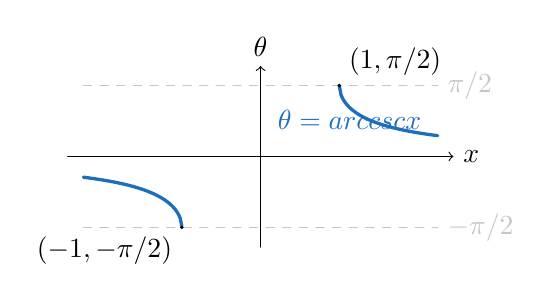
\begin{tikzpicture}[scale=1.0, line cap=round, line join=round]
  \definecolor{trigblue}{RGB}{30,110,190}
  \draw[->] (-2.45,0)--(2.45,0) node[right] {$x$};
  \draw[->] (0,-1.15)--(0,1.15) node[above] {$\theta$};
  \draw[gray!45,dashed] (-2.25,0.9)--(2.25,0.9) node[right] {$\pi/2$};
  \draw[gray!45,dashed] (-2.25,-0.9)--(2.25,-0.9) node[right] {$-\pi/2$};
  \draw[very thick,trigblue,domain=1:2.25,samples=60]
    plot ({\x},{0.9*asin(1/\x)/90});
  \draw[very thick,trigblue,domain=-2.25:-1,samples=60]
    plot ({\x},{0.9*asin(1/\x)/90});
  \fill (1,0.9) circle (0.025) node[above right] {$(1,\pi/2)$};
  \fill (-1,-0.9) circle (0.025) node[below left] {$(-1,-\pi/2)$};
  \node[trigblue] at (1.13,0.47) {$\theta=\operatorname{arccsc} x$};
\end{tikzpicture}
\end{center}


\begin{definitionbox}{Definition}
\begin{definition}[Inverse cosecant]
\label{def:inverse-cosecant}
The \emph{inverse cosecant} function is the inverse of cosecant after cosecant
is restricted to $[-\pi/2,\pi/2]\setminus\{0\}$. It is denoted by $\operatorname{arccsc}$
or $\csc^{-1}$ and has domain $(-\infty,-1]\cup[1,\infty)$ and range
$[-\pi/2,\pi/2]\setminus\{0\}$.
\[
  \operatorname{arccsc} x=\theta
  \quad\Longleftrightarrow\quad
  \csc\theta=x
  \quad\text{and}\quad
  -\frac{\pi}{2}\leq\theta\leq\frac{\pi}{2},\ \theta\neq 0.
\]
\end{definition}
\end{definitionbox}
\begin{remark*}[Standard quantified statement]
For every admissible input satisfying the hypotheses of the statement, the
displayed definition or assertion holds in the stated domain.
\end{remark*}

\begin{remark*}[Interpretation]
The statement records the named trigonometric object or identity together with
its intended domain of use.
\end{remark*}

\begin{remark*}[Domain and range]
The cosecant function has domain
$\mathbb{R}\setminus\{k\pi:k\in\mathbb{Z}\}$ and range
$(-\infty,-1]\cup[1,\infty)$. The inverse cosecant function reverses the
principal restricted cosecant function.
\end{remark*}
\begin{dependencies}
\begin{itemize}
  \item \hyperref[def:extended-cosecant]{Extended cosecant}
  \item \hyperref[def:radian-measure]{Radian measure}
\end{itemize}
\end{dependencies}

\begin{theorembox}{Theorem}
\begin{theorem}[Principal inverse cosecant identities]
\label{thm:inverse-cosecant-identities}
For every $x\in(-\infty,-1]\cup[1,\infty)$,
\[
  \csc(\operatorname{arccsc} x)=x.
\]
For every $\theta\in[-\pi/2,\pi/2]\setminus\{0\}$,
\[
  \operatorname{arccsc}(\csc\theta)=\theta.
\]
\end{theorem}
\end{theorembox}
\begin{remark*}[Interpretation]
The statement records the named trigonometric object or identity together with
its intended domain of use.
\end{remark*}

\begin{remark*}[Standard quantified statement]
$\forall x\in(-\infty,-1]\cup[1,\infty)$, $\csc(\operatorname{arccsc} x)=x$, and
$\forall \theta\in[-\pi/2,\pi/2]\setminus\{0\}$,
$\operatorname{arccsc}(\csc\theta)=\theta$.
\end{remark*}
\begin{dependencies}
\begin{itemize}
  \item \hyperref[def:inverse-cosecant]{Inverse cosecant}
\end{itemize}
\end{dependencies}
